\documentclass{article}
\usepackage[spanish]{babel}
\usepackage{amssymb, amsmath}
\usepackage{graphicx}
\usepackage{hyperref}
\hypersetup{
colorlinks=true,
citecolor=blue,
urlcolor=blue
}
\author{Lucas Aljarilla Sanchez}
\title{Introducción a la Investigación Operativa}
\begin{document}
\maketitle
\begin{abstract}
Breve introducción a la investigación operativa para aquelos que quieren saber un poco más de este mundillo. Veremos cómo surgió, los tipos que hay y sus usos actuales. Para más información sobre este trabajo mirar la url: \url{https://github.com/Lucasal2000/proyecto_final} 
\end{abstract}
 \vfill
\textbf{Palabras clave}
\begin{itemize}
\item  \underline{modelo matemático}: formula matemática empleada para expresar relaciones, proposiciones sustantivas de hechos, variables, parámetros, entidades y relaciones entre variables de las operaciones, para estudiar comportamientos de sistemas complejos ante situaciones difíciles de observar en la realidad.
\item  \underline{modelo determinístico}: modelo matemático donde las condiciones iniciales producen invariablemente los mismos resultados.
\item  \underline{modelo estocástico}: modelo matemático con un comportamiento no determinístico, por lo que su resultado es aleatorio.
\item  \underline{sistema}: un conjunto de elementos relacionados entre sí que funciona como un todo, en nuestro caso el sistema es el modelo con sus respectivas restricciones. 
\end{itemize}

\section{Introducción}

Muchos os preguntareis qué es eso de la investigación operativa. Bien, según Ackoff, Arnoff y Churchman: "La investigación operativa es la aplicación, por grupos interdisciplinarios, del método científico a problemas relacionados con el control de las organizaciones o sistemas (Hombre-Máquina) a fin de que se produzcan soluciones que mejor sirvan a los objetivos de toda la organización."

En resumidas cuentas, es la rama de las matemáticas que se ocupa de la toma de decisiones óptimas y de modelar sistemas determinísticos y estocásticos que se originan en la vida real.

\section{Etapas de un problema de investigación operativa}

\subsection{Formulación del problema}
Estudiar el sistema que se va a analizar:Definir el problema, especificar los objetivos y las limitaciones bajo las cuales opera el sistema que se modeliza.
\subsection{Construcción del modelo}
Modelo: Representación idealizada del sistema que reproduce la realidad de la forma más fiel posible, tratando de entender cómo se comporta el mundo real.
\subsection{Obtención de solución}
Obtener una solución óptima teniendo en cuenta que estas soluciones son óptimas sólo respecto al modelo utilizado.
\subsection{Validación del modelo}
Comprobar si el modelo propuesto hace lo que se supone que debe hacer.
¿Proporciona una predicción razonable del comportamiento del sistema que se está estudiando?
\subsection{Puesta en practica}
Poner en práctica la solución final.
\section{Modelos de investigación operativa}
\begin{minipage}[b]{0.5\linewidth}
\begin{itemize}
\item \textbf{Determinísticos}
\item Análisis de redes
\item Programación lineal multiobjetivo
\item Programación lineal
\end{itemize}
    \end{minipage} 
    \begin{minipage}[b]{0.5\linewidth} 
\begin{itemize}
\item \textbf{Estocásticos}
\item Teoria de intervalos
\item Teoría de juegos
\item Teoria de colas
\end{itemize}    
\end{minipage}

\section{Aplicaciones de la investigación operativa}
La investigación operativa es usada para un montón de cosas en nuestro día a día, pero unos de los ejemplos más famosos y más estudiados son: el problema de la dieta, el problema de transporte y el problema de cartera de valores.

\section{Programación lineal}
Dentro de la investigación operativa encontramos los problemas de programación lineal.

Un problema de programación lineal es un programa matemático en el cual la función objetivo es lineal en las variables de decisión y cada restricción es una desigualdad lineal. Además tiene una restricción de signo; es decir, las variables de decisión son no negativas. Vamos a ver un pequeño ejemplo:

\textbf{Ejemplo}
\begin{equation}
\begin{split}
MaxZ&=2x_1+2x_2\\
s.a.~&-x_1+x_2\leq 2\\
&x_1+2x_2\leq 6\\
&2x_1+x_2\leq 6\\
&x_1,x_2\geq 0
\end{split}
\end{equation}
\begin{center}
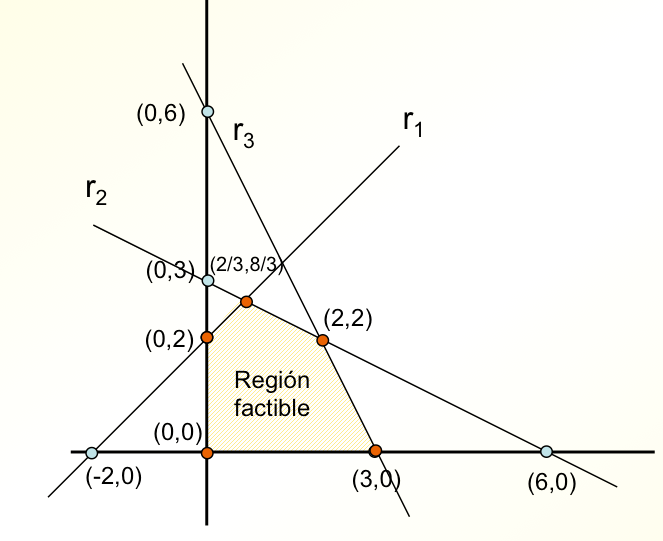
\includegraphics[width=.70\textwidth]{ej_grafi.png} \\
\end{center}

\begin{center}
\begin{tabular}{ c | c }
Soluciones ($x_1,x_2$)  & Valor de la función objetivo (Z) \\ \hline 
(0,0) & Z=0 \\
(0,2) & Z=2 \\
(2/3,8/3) & Z=4 \\
(2,2) & Z=6 \\
(3,0) & Z=6
\end{tabular}
\end{center}



\end{document}